\documentclass[12pt]{article} % use larger type; default would be 10pt
\usepackage[czech]{babel}
\usepackage[utf8]{inputenc} % set input encoding (not needed with XeLaTeX)

%%% PAGE DIMENSIONS
\usepackage{geometry} % to change the page dimensions
% \usepackage[left=2cm,right=2cm,top=2cm,bottom=2cm]{geometry}
\geometry{a4paper}
% \geometry{margin=2in} % for example, change the margins to 2 inches all round
% \geometry{landscape} % set up the page for landscape

\usepackage{graphicx} % support the \includegraphics command and options
\usepackage{wrapfig} % support the wrapfigure section

\usepackage{hyperref} % links in \tableofcontents
\hypersetup{
	colorlinks,
	citecolor=black,
	filecolor=black,
	linkcolor=black,
	urlcolor=black
}

% \usepackage[parfill]{parskip} % Activate to begin paragraphs with an empty line rather than an indent

%%% PACKAGES
\usepackage{booktabs} % for much better looking tables
\usepackage{array} % for better arrays (eg matrices) in maths
%\usepackage{paralist} % very flexible & customisable lists (eg. enumerate/itemize, etc.)
\usepackage{verbatim} % adds environment for commenting out blocks of text & for better verbatim
\usepackage{subfig} % make it possible to include more than one captioned figure/table in a single float
% These packages are all incorporated in the memoir class to one degree or another...
\usepackage{tikz} % graphs
\usepackage{pgfplots}
\usepackage{float}

%%% HEADERS & FOOTERS
\usepackage{fancyhdr} % This should be set AFTER setting up the page geometry
\pagestyle{fancy} % options: empty , plain , fancy
\renewcommand{\headrulewidth}{0pt} % customise the layout...
\lhead{}\chead{}\rhead{}
\lfoot{}\cfoot{\thepage}\rfoot{}

%%% SECTION TITLE APPEARANCE
\usepackage{sectsty}
\allsectionsfont{\sffamily\mdseries\upshape} % (See the fntguide.pdf for font help)
% (This matches ConTeXt defaults)

%%% ToC (table of contents) APPEARANCE
\usepackage[nottoc,notlof,notlot]{tocbibind} % Put the bibliography in the ToC
\usepackage[titles,subfigure]{tocloft} % Alter the style of the Table of Contents
\renewcommand{\cftsecfont}{\rmfamily\mdseries\upshape}
\renewcommand{\cftsecpagefont}{\rmfamily\mdseries\upshape} % No bold!
\newcommand{\bigsize}{\fontsize{35pt}{20pt}\selectfont}

%%% END Article customizations

\begin{document}
\begin{titlepage}
	
\includegraphics[scale=0.7]{logo.jpg}
	\vspace*{\fill}
	\begin{center}
		\textsc{\LARGE Katedra technologií a měření}\\[0.3cm]
		\textsc{\LARGE \bigsize Fyzikální elektronika}\\[0.3cm]
		\textsc{\LARGE Měření usměrňovačů s polovodičovými diodami}\\[1cm]
		Martin Zlámal \\
		Josef Sedlák \\[1cm]
		{\small\em \ Datum měření 7. října 2013 } \\
		{\small\em \copyright \ Datum poslední revize \today } \\
		\LaTeX
	\end{center}
	\vspace*{\fill}
\end{titlepage}
\tableofcontents
\listoffigures
\listoftables
\newpage

\section{Zadání}
\begin{enumerate}
\item Zapojte postupně jednotlivé typy usměrňovačů. Pro každý typ usměrňovače
zaznamenejte co nejpřesněji časové průběhy výstupních napětí za následujících
podmínek:
	\begin{itemize}
		\item pro odporovou zátěž $R_Z = 30 \Omega$ bez vyhlazovacího kondenzátoru a poté
postupně pro 3 různé kondenzátory
		\item pro odporovou zátěž $R_Z = 100 \Omega$ bez vyhlazovacího kondenzátoru a poté
postupně pro 3 různé kondenzátory
	\end{itemize}
\item U všech průběhů určete velikost zvlnění výstupního napětí $\Delta U [V]$ a vypočítejte činitel zvlnění $p [\%]$.
\item V závěru zhodnoťte vliv zapojení usměrňovače, velikosti zatěžovacího odporu $R_Z$ a
velikosti kapacity vyhlazovacího kondenzátoru na špičkovou hodnotu výstupního
napětí $U_{max}$ a míru zvlnění.
\end{enumerate}

\section{Katalogové parametry měřených součástek}
Při měření byla jako usměrňovací dioda použita 4x BYW96.
\begin{table}[H]
\caption{Mezní hodnoty diody BYW96}
\begin{tabular}{|c|c|}
\hline 
Mezní hodnota proudu v propustném směru $I_F$ & max. $3 A$ \\ 
\hline 
Mezní hodnota proudu v závěrném směru $I_R$ & max. $1 uA$ \\ 
\hline 
Průrazné napětí v závěrném směru $V_{(BR)R}$ & max. $900 V$ \\ 
\hline 
Obnovovací čas $t_{rr}$ & $300 ns$ \\ 
\hline 
\end{tabular} 
\end{table}

\section{Schéma zapojení}
\begin{figure}[H]
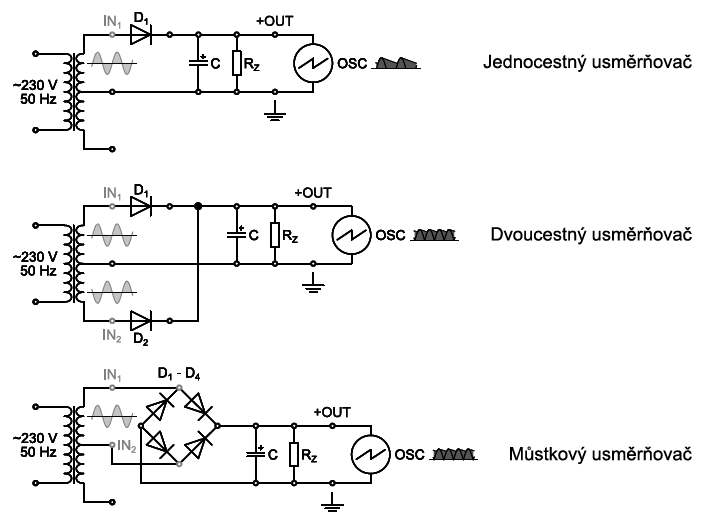
\includegraphics[scale=0.8]{schema.png}
\caption{Schémata zapojení základních typů usměrňovačů}
\end{figure}

\section{Jednocestný usměrňovač}
\begin{figure}[H]
\center
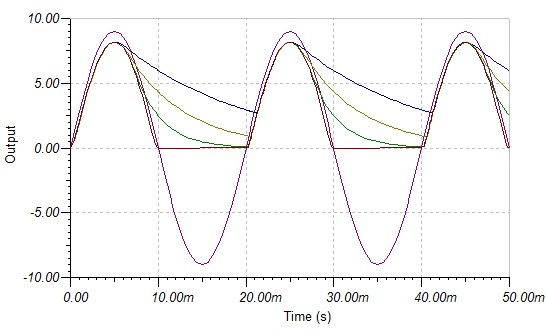
\includegraphics[scale=0.7]{jednocestny30.jpg}
\caption{Tvary průběhů jednocestného usměrňovače pro $R_Z = 30\Omega$}
\end{figure}

\begin{figure}[H]
\center
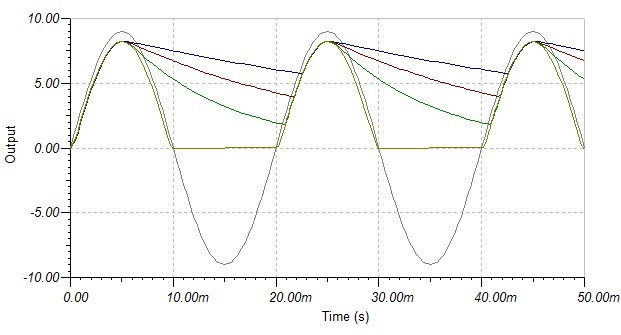
\includegraphics[scale=0.7]{jednocestny100.jpg}
\caption{Tvary průběhů jednocestného usměrňovače pro $R_Z = 100\Omega$}
\end{figure}

\subsection{Naměřené a vypočtené hodnoty}
\begin{table}[H]
\caption{Jednocestný usměrňovač s $R_Z=30\Omega$}
\begin{tabular}{|c|c|c|c|c|}
\hline 
• & bez kondenzátoru & $C_1 = 100uF$ & $C_2 = 220uF$ & $C_3 = 470uF$ \\ 
\hline 
$U_{min} [V]$ & 0 & 0 & 0,50 & 2,68 \\ 
\hline 
$U_{max} [V]$ & 8,24 & 8,32 & 9,40 & 8,00 \\ 
\hline 
$U [V]$ & 4,13 & 4,19 & 4,67 & 5,10 \\ 
\hline 
$U_0 [V]$ & 2,51 & 2,80 & 3,95 & 4,82 \\ 
\hline 
$\Delta U [V]$ & 8,24 & 8,32 & 8,90 & 5,32 \\ 
\hline 
$p [\%]$ & 64,5 & 49,6 & 18,2 & 5,8 \\ 
\hline 
\end{tabular}
\end{table}

\begin{table}[H]
\caption{Jednocestný usměrňovač s $R_Z=100\Omega$}
\begin{tabular}{|c|c|c|c|c|}
\hline 
• & bez kondenzátoru & $C_1 = 100uF$ & $C_2 = 220uF$ & $C_3 = 470uF$ \\ 
\hline 
$U_{min} [V]$ & 0 & 0,70 & 3,92 & 5,36 \\ 
\hline 
$U_{max} [V]$ & 8,72 & 8,72 & 8,72 & 8,58 \\ 
\hline 
$U [V]$ & 4,38 & 4,91 & 6,38 & 7,15 \\ 
\hline 
$U_0 [V]$ & 2,68 & 4,08 & 6,18 & 7,10 \\ 
\hline 
$\Delta U [V]$ & 8,72 & 8,02 & 4,80 & 3,22 \\ 
\hline 
$p [\%]$ & 63,4 & 20,3 & 3,2 & 0,7 \\ 
\hline 
\end{tabular}
\end{table}

Kde zvlnění výstupního napětí $\Delta U$:
\begin{equation}
\Delta U = U_{max} - U_{min} = 8,24 - 0 = 8,24 V
\end{equation}
Činitel zvlnění $p$:
\begin{equation}
p = \sqrt{\left( \frac{U}{U_0} -1 \right)^2} \cdot 100 = \sqrt{\left( \frac{4,13}{2,51} -1 \right)^2} \cdot 100 = 64,5\%
\end{equation}
Stejným způsobem se vypočítává zvlnění výstupního napětí a činitel tohoto zvlnění u všech dalších obvodů.

\section{Dvoucestný usměrňovač}
\begin{figure}[H]
\center
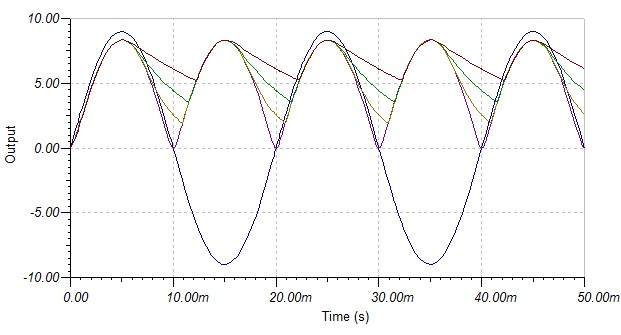
\includegraphics[scale=0.7]{dvoucestny30.jpg}
\caption{Tvary průběhů dvoucestného usměrňovače pro $R_Z = 30\Omega$}
\end{figure}

\begin{figure}[H]
\center
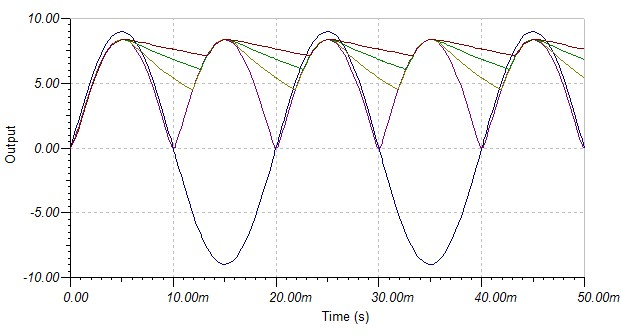
\includegraphics[scale=0.7]{dvoucestny100.jpg}
\caption{Tvary průběhů dvoucestného usměrňovače pro $R_Z = 100\Omega$}
\end{figure}

\subsection{Naměřené a vypočtené hodnoty}
\begin{table}[H]
\caption{Dvoucestný usměrňovač s $R_Z=30\Omega$}
\begin{tabular}{|c|c|c|c|c|}
\hline 
• & bez kondenzátoru & $C_1 = 100uF$ & $C_2 = 220uF$ & $C_3 = 470uF$ \\ 
\hline 
$U_{min} [V]$ & 0 & 1,27 & 3,47 & 4,47 \\ 
\hline 
$U_{max} [V]$ & 8,35 & 8,50 & 8,24 & 8,28 \\ 
\hline 
$U [V]$ & 5,80 & 5,87 & 6,31 & 6,68 \\ 
\hline 
$U_0 [V]$ & 5,10 & 5,35 & 6,11 & 6,62 \\ 
\hline 
$\Delta U$ & 8,35 & 7,23 & 4,77 & 3,81 \\ 
\hline 
$p [\%]$ & 13,7 & 9,7 & 3,3 & 0,9 \\ 
\hline 
\end{tabular}
\end{table}

\begin{table}[H]
\caption{Dvoucestný usměrňovač s $R_Z=100\Omega$}
\begin{tabular}{|c|c|c|c|c|}
\hline 
• & bez kondenzátoru & $C_1 = 100uF$ & $C_2 = 220uF$ & $C_3 = 470uF$ \\ 
\hline 
$U_{min} [V]$ & 0 & 3,39 & 6,04 & 7,15 \\ 
\hline 
$U_{max} [V]$ & 8,75 & 8,99 & 9,98 & 8,69 \\ 
\hline 
$U [V]$ & 6,13 & 6,64 & 7,54 & 7,87 \\ 
\hline 
$U_0 [V]$ & 5,39 & 6,40 & 7,49 & 7,86 \\ 
\hline 
$\Delta U$ & 8,75 & 5,60 & 3,94 & 1,54 \\ 
\hline 
$p [\%]$ & 13,7 & 3,8 & 0,7 & 0,1 \\ 
\hline 
\end{tabular}
\end{table}

\section{Můstkový usměrňovač}
\begin{figure}[H]
\center
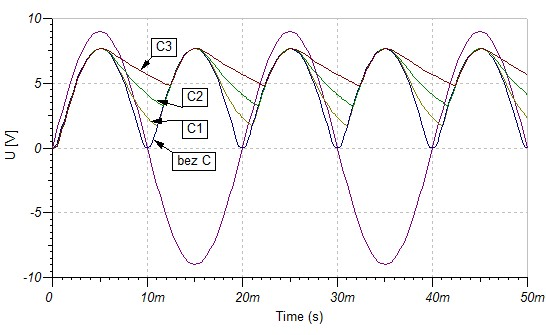
\includegraphics[scale=0.7]{mustkovy30.jpg}
\caption{Tvary průběhů můstkového usměrňovače pro $R_Z = 30\Omega$}
\end{figure}

\begin{figure}[H]
\center
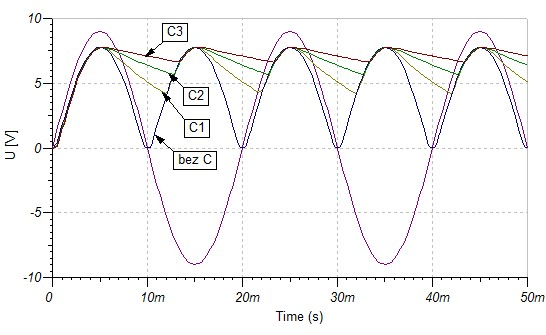
\includegraphics[scale=0.7]{mustkovy100.jpg}
\caption{Tvary průběhů můstkového usměrňovače pro $R_Z = 100\Omega$}
\end{figure}

\subsection{Naměřené a vypočtené hodnoty}
\begin{table}[H]
\caption{Můstkový usměrňovač s $R_Z=30\Omega$}
\begin{tabular}{|c|c|c|c|c|}
\hline 
• & bez kondenzátoru & $C_1 = 100uF$ & $C_2 = 220uF$ & $C_3 = 470uF$ \\ 
\hline 
$U_{min} [V]$ & 0 & 0,90 & 3,08 & 4,56 \\ 
\hline 
$U_{max} [V]$ & 8,63 & 7,52 & 7,45 & 7,27 \\ 
\hline 
$U [V]$ & 5,15 & 5,19 & 5,62 & 6,0 \\ 
\hline 
$U_0 [V]$ & 4,42 & 4,68 & 5,43 & 5,95 \\ 
\hline 
$\Delta U$ & 8,63 & 6,62 & 4,37 & 2,71 \\ 
\hline 
$p [\%]$ & 16,5 & 10,9 & 3,5 & 0,8 \\ 
\hline 
\end{tabular}
\end{table}

\begin{table}[H]
\caption{Můstkový usměrňovač s $R_Z=100\Omega$}
\begin{tabular}{|c|c|c|c|c|}
\hline 
• & bez kondenzátoru & $C_1 = 100uF$ & $C_2 = 220uF$ & $C_3 = 470uF$ \\ 
\hline 
$U_{min} [V]$ & 0 & 3,68 & 5,42 & 6,47 \\ 
\hline 
$U_{max} [V]$ & 8,01 & 8,07 & 8,01 & 7,76 \\ 
\hline 
$U [V]$ & 5,51 & 5,78 & 6,86 & 7,14 \\ 
\hline 
$U_0 [V]$ & 4,75 & 6,01 & 6,82 & 7,13 \\ 
\hline 
$\Delta U$ & 8,01 & 4,39 & 2,59 & 1,29 \\ 
\hline 
$p [\%]$ & 16,0 & 3,9 & 0,5 & 0,1 \\ 
\hline 
\end{tabular}
\end{table}

\section{Závěr}
Jednocestné zapojení usměrňovače je sice nejjednodušší, ale má také celou řadu nevýhod. Hlavní nevýhodou je to, že usměňuje pouze jednu půlvlnu vstupního signálu, tzn. vyhlazovací kondenzátor má celou dobu půl periody na to, aby se vybíjel. To se negativně podepisuje jak na zvlnění výstupního napětí, tak  na činiteli zvlnění.

Dvoucestný a můstkový usměrňovač dělají v konečném důsledku to samé, tedy usměrňují obě půlvlny vstpuního signálu. Zásadní rozdíl mezi dvoucestným a můstkovým zapojením je ten, že u můstkového zapojení teče proud přes dvě diody a vzniká tak dvoujnásobný úbytek napětí než u dvoucestného zapojení. To je dobře vidět na aplitudě signálů znázorněných na grafech. Dvoucestný usměrňovač má naopak nevýhodu v tom, že je potřeba transformátor s vyvedeným středem.

Z výsledků měření vyplývá, že čím je vyhlazovací kondenzátor větší, tím je schopen akumulovat více energie a dochází k většímu vyhlazení (k menšímu zvlnění). Větší hodnota rezistoru také přispívá k lepšímu vyhlazení.

\end{document}
